% mnras_template.tex
%
% LaTeX template for creating an MNRAS paper
%
% v3.0 released 14 May 2015
% (version numbers match those of mnras.cls)
%
% Copyright (C) Royal Astronomical Society 2015
% Authors:
% Keith T. Smith (Royal Astronomical Society)

% Change log
%
% v3.0 May 2015
%    Renamed to match the new package name
%    Version number matches mnras.cls
%    A few minor tweaks to wording
% v1.0 September 2013
%    Beta testing only - never publicly released
%    First version: a simple (ish) template for creating an MNRAS paper

%%%%%%%%%%%%%%%%%%%%%%%%%%%%%%%%%%%%%%%%%%%%%%%%%%
% Basic setup. Most papers should leave these options alone.
\documentclass[a4paper,fleqn,usenatbib]{mnras}

% MNRAS is set in Times font. If you don't have this installed (most LaTeX
% installations will be fine) or prefer the old Computer Modern fonts, comment
% out the following line
\usepackage{newtxtext,newtxmath}
% Depending on your LaTeX fonts installation, you might get better results with one of these:
%\usepackage{mathptmx}
%\usepackage{txfonts}

% Use vector fonts, so it zooms properly in on-screen viewing software
% Don't change these lines unless you know what you are doing
\usepackage[T1]{fontenc}
\usepackage{ae,aecompl}


%%%%% AUTHORS - PLACE YOUR OWN PACKAGES HERE %%%%%

% Only include extra packages if you really need them. Common packages are:
\usepackage{graphicx}    % Including figure files
\usepackage{amsmath}    % Advanced maths commands
\usepackage{amssymb}    % Extra maths symbols

\usepackage{todonotes}
\graphicspath{{img/}}   % Set image path

%%%%%%%%%%%%%%%%%%%%%%%%%%%%%%%%%%%%%%%%%%%%%%%%%%

%%%%% AUTHORS - PLACE YOUR OWN COMMANDS HERE %%%%%

% Please keep new commands to a minimum, and use \newcommand not \def to avoid
% overwriting existing commands. Example:
%\newcommand{\pcm}{\,cm$^{-2}$}    % per cm-squared
\newcommand{\Sun}[0]{\ensuremath{_{\odot}}}
\renewcommand{\deg}{\ensuremath{^{\circ}}}


%%%%%%%%%%%%%%%%%%%%%%%%%%%%%%%%%%%%%%%%%%%%%%%%%%

%%%%%%%%%%%%%%%%%%% TITLE PAGE %%%%%%%%%%%%%%%%%%%

% Title of the paper, and the short title which is used in the headers.
% Keep the title short and informative.
\title[Auriga GCS]{The Globular Cluster System of the Auriga Simulations}

% The list of authors, and the short list which is used in the headers.
% If you need two or more lines of authors, add an extra line using \newauthor
\author[T. L. R. Halbesma et al.]{
Timo L. R. Halbesma,$^{1}$\thanks{E-mail: Halbesma@MPA-Garching.MPG.DE}
Simon D. M. White,$^{1}$
\\
% List of institutions
$^{1}$Max-Planck-Institut f\"ur Astrophysik, Postfach 1317, D-85741 Garching, Germany\\
}

% These dates will be filled out by the publisher
\date{Accepted XXX. Received YYY; in original form ZZZ}

% Enter the current year, for the copyright statements etc.
\pubyear{2019}

% Don't change these lines
\begin{document}
\label{firstpage}
\pagerange{\pageref{firstpage}--\pageref{lastpage}}
\maketitle

% Abstract of the paper
\begin{abstract}
We investigate whether the galaxy formation model used for the Auriga simulations 
can produce a realistic globular cluster population at redshift zero. We compare
properties of the simulated star particles in selected Auriga haloes with
catalogues of observations of the Milky Way globular cluster population available
in the literature. We find that the Auriga simulations produce sufficient mass
at radii and metallicities that are typical for the MW GCS, although we observe
a varying mass-excess for the different $R_{\text{GC}}$-[Fe/H] bins. This implies
different values for the combined product of the bound cluster formation efficiency
and the globular cluster disruption rate.
\end{abstract}

% Select between one and six entries from the list of approved keywords.
% Don't make up new ones.
\begin{keywords}
methods: numerical -- galaxies: formation -- galaxies: star clusters: general.
\end{keywords}

%%%%%%%%%%%%%%%%%%%%%%%%%%%%%%%%%%%%%%%%%%%%%%%%%%

%%%%%%%%%%%%%%%%% BODY OF PAPER %%%%%%%%%%%%%%%%%%

\section{Introduction}
\todo[inline]{Paragraph: General introduction of GCs}
\begin{itemize}
    \item ``GCs among oldest astrophysical objects. GCs form in the early Universe in highest density peaks \citep[e.g.][]{2005MNRAS.364..367D, 2009ApJ...706L.192B}''
    \item ``Hence, they witness most of the formation and evolution processes of galaxies, and can be used to probe them'' \citep{2006ARA&A..44..193B}
    \item ``colour bimodality, blue and red clusters \citep[e.g.][]{1985ApJ...293..424Z, 1999AJ....118.1526G, 2001AJ....121.2974L, 2006ApJ...639...95P}
    \item ``blue metal-poor (with distribution peaking at [Fe/H] $\approx -1.5$ for the Milky Way), no sign of rotation as a population (..) more metal-rich (peak at [Fe/H] $\approx -0.5$ in the Milky  Way) more spatially concentrated and rotating with the galaxy.'' \citep{1996AJ....112.1487H}
\end{itemize}


\todo[inline]{Paragraph: ``Bimodality suggests two formation mechanisms''}
\begin{itemize}
    \item ``Blue clusters from in early Universe in galaxies that merge later. In (wet) merger process starbursts generate red population \cite{1992ApJ...384...50A, 1987nngp.proc...18S}''
    \item ``\citet{1997AJ....113.1652F} propose instead that blue globulars form when the protogalaxy itself collapses, in a metal-poor and turbulence media. The red population would form later, once the galactic disc has settled. The formation of globular clusters would then be a multiphase process, with the first phase being interrupted possibly by cosmic reionization \citep{2002MNRAS.333..383B}.''
    \item ``\citet{2005ApJ...623..650K, 2014ApJ...796...10L} advocate
that major mergers are at the origin of both sub-populations: blue
clusters form during early mergers (z > 4) while the red ones appear
in mergers at lower redshifts (even after z = 1). Although, this
scenario, combined with star formation enhancement in mergers,
seems appropriate in dense galactic environment leading to the
assembly of massive elliptical galaxies, like in the Virgo Cluster
as tested by \citet{2014ApJ...796...10L}, it does not apply to Milky Way-
like systems where no recent major merger took place (Wyse 2001;
Deason et al. 2013; Ruchti et al. 2014, 2015).
\item ``\citet{1998ApJ...501..554C} argue that red clusters form in situ while the blue ones are accreted, either via merging satellite galaxies, or by tidal capture of the clusters themselves \citep[see also][]{2013ApJ...762...39T}.''
\end{itemize}


\todo[inline]{Work of other groups}
\begin{itemize}
\item Origin of the Milky Way globular clusters \citep{2017MNRAS.465.3622R}
\item GCs in FIRE \citep{2018MNRAS.474.4232K}
\item EMOSAICS project \citep{2018MNRAS.475.4309P}
\item Origin of GC bimodality? \citep{2018MNRAS.479..200F}
\item \textit{GAIA} DR2: GC kinematics \citep{2018A&A...616A..12G}, Dating GC Tidal Disruption \citep{2018ApJ...859L..13B}
\item GC in N-body simulation \citep{2018ApJ...861...69C}
\item Tangentially related? role of GC mass evolution on stream properties \citep{2018MNRAS.474.2479B}
\item GC formation from dwarfs to giants \citep{2018MNRAS.480.2343C}
\item GC contribution to EOR \citep{2018MNRAS.479..332B}
\item Early Universe supermassive star / GC formation \citep{2018MNRAS.478.2461G}
\item GC formation in cold filaments \citep{2018ApJ...861..148M}
\item GC formation in high-redshift dwarf galaxies \citep{2018MNRAS.477..480Z}
\item GCs in MW outer region \citep{2017arXiv170804542P}
\end{itemize}

\section{Methodology and definitions}
\label{sec:methods}
\subsection{The Auriga Simulations}
\label{sec:auriga}
We use the Auriga \citep[][hereafter G17]{2017MNRAS.467..179G} simulations, a suite of high-resolution cosmological zoom simulations ran with a galaxy formation model that produces realistic Milky Way-like galaxies at redshift $z=0$. The simulations are performed with \textsc{arepo} \citep{2010MNRAS.401..791S, 2016MNRAS.455.1134P} that solves the magnetohydrodynamical equations on a moving mesh. See G17 for further details; here we briefly summarise the relevant properties.
\todo[inline]{Paragraph: Auriga boilerplate, paraphrased}

\todo[inline]{What is the star formation density threshold?}


\subsection{Definition of stellar halo}
\todo[inline]{Possibly also relevant here. See \citet{2018arXiv180407798M}.}


\subsection{Definition of accreted and in-situ component}
\todo[inline]{Possibly also relevant here. See \citet{2018arXiv180407798M}.}



\section{Comparison with observations}
\label{sec:observations}

\begin{figure*}
    \includegraphics[width=\textwidth]{{Au4-24_GCS_250_10}.pdf}
    \caption{TODO: combine upper left and mid left panel, remove upper right panel,
             remove lower panels (because mid right panel already shows the 
             relevant info). The point of this figure is to compare metallicity 
             distribution and radial distribution}
    \label{fig:FeH_Rcs_MWvsAu424_1D}
\end{figure*}


\begin{figure*}
    \includegraphics[width=\textwidth]{{Au4-24_FeH_vs_Rgc}.pdf}
    \caption{Comparison of [Fe/H] and galactocentric radius of the Milky Way GCS
             (red dots) with the star particles in Au4-24. TODO: only show the
             panel on the right-hand side. TODO: include details of exactly which
             star particles are shown. TODO: generate the same figure but color-coded
             by mass?}
    \label{fig:FeH_Rcs_MWvsAu424_2D}
\end{figure*}


\begin{figure*}
    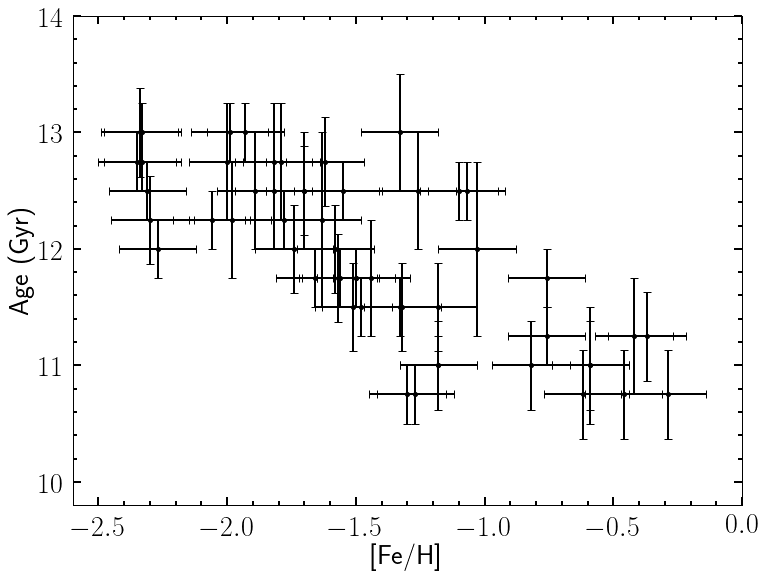
\includegraphics[width=\columnwidth]{vandenBergh2013.png}
    \includegraphics[width=\columnwidth]{{Au4-24_Renaud2017_figure8}.png}
    \caption{TODO: add observed age-FeH data points \citep{2013ApJ...775..134V}
             to simulation plot, investigate starbursts by making pictures of
             these events, check if the observed data set shows a representative
             sample of the MW GCS, fix overlapping axes labels}
    \label{fig:bla}
\end{figure*}
\begin{figure}
    \includegraphics[width=\columnwidth]{{Au4-24_Renaud2017_figure6}.png}
    \caption{}
    \label{fig:bla}
\end{figure}






\section{Discussion}
\label{sec:discussion}


\section{Summary and conclusions}
\label{sec:summary}


\section*{Acknowledgements}
TLRH acknowledges support from the International Max-Planck Research School (IMPRS) on Astrophysics.

\todo[inline]{Check Auriga boilerplate that we need to acknowledge}
RG and VS acknowledge support by the DFG Research Centre SFB-881 `The
Milky Way System' through project A1. This work has also been
supported by the European Research Council under ERC-StG grant
EXAGAL- 308037. Part of the simulations of this paper used the
SuperMUC system at the Leibniz Computing Centre, Garching,
under the project PR85JE of the Gauss Centre for Supercomputing.
This work used the DiRAC Data Centric system at Durham
University, operated by the Institute for Computational Cosmology
on behalf of the STFC DiRAC HPC Facility `www.dirac.ac.uk'.
This equipment was funded by BIS National E-infrastructure capital 
grant ST/K00042X/1, STFC capital grant ST/H008519/1 and
STFC DiRAC Operations grant ST/K003267/1 and Durham University. 
DiRAC is part of the UK National E-Infrastructure.

%%%%%%%%%%%%%%%%%%%%%%%%%%%%%%%%%%%%%%%%%%%%%%%%%%

%%%%%%%%%%%%%%%%%%%% REFERENCES %%%%%%%%%%%%%%%%%%

% The best way to enter references is to use BibTeX:

\bibliographystyle{mnras}
\bibliography{AurigaGCS} % if your bibtex file is called example.bib


% Alternatively you could enter them by hand, like this:
% This method is tedious and prone to error if you have lots of references
%\begin{thebibliography}{99}
%\bibitem[\protect\citeauthoryear{Author}{2012}]{Author2012}
%Author A.~N., 2013, Journal of Improbable Astronomy, 1, 1
%\bibitem[\protect\citeauthoryear{Others}{2013}]{Others2013}
%Others S., 2012, Journal of Interesting Stuff, 17, 198
%\end{thebibliography}

%%%%%%%%%%%%%%%%%%%%%%%%%%%%%%%%%%%%%%%%%%%%%%%%%%

%%%%%%%%%%%%%%%%% APPENDICES %%%%%%%%%%%%%%%%%%%%%

\appendix

\section{Some extra material}

If you want to present additional material which would interrupt the flow of the main paper,
it can be placed in an Appendix which appears after the list of references.

%%%%%%%%%%%%%%%%%%%%%%%%%%%%%%%%%%%%%%%%%%%%%%%%%%


% Don't change these lines
\bsp    % typesetting comment
\label{lastpage}
\end{document}

% End of mnras_template.tex
